
\documentclass{article}

%%%%%%%%%%%%%%%%%%%%%%%%%%%%%%%%%%%%%%%%%%%%%%%%%%%%%%%%%%%%%%%%
\usepackage[utf8]{inputenc}
\usepackage[top=3cm, bottom=3cm, left=2.5cm, right=2.5cm]{geometry}
\usepackage{graphicx}
\usepackage{float}
\usepackage[colorlinks=true, linkcolor=blue]{hyperref}
\usepackage{amsmath,amsthm,amsfonts,amssymb}
\usepackage{wrapfig}

\usepackage{Sweave}
\begin{document}
%%%%%%%%%%%%%%%%%%%%%%%%%%%%%%%%%%%%%%%%%%%%%%%%%%%%%%%%%%%%%%%%
  
  
\Sconcordance{concordance:p1.tex:p1.Rnw:%
1 12 1 1 0 1 1 1 19 56 1 1 19 1 2 1 0 2 1 1 5 7 0 1 2 1 1 1 5 1 2 6 1 1 %
2 1 0 2 1 1 5 8 0 1 3 1 1 1 5 1 2 6 1 1 2 1 0 2 1 1 7 5 0 1 7 5 0 1 7 9 %
0 1 3 2 1 1 5 1 2 11 1}


%%%%%%%%%%%%%%%%%%%%%%%%%%%%%%%%%%%%%%%%%%%%%%%%%%%%%%%%%%%%%%%%
  % strona tytulowa
\title{Statistical packages - report 2}
\author{Urszula Grochocińska, Marcin Mazurkiewicz}
\maketitle
\tableofcontents 


%%%%%%%%%%%%%%%%%%%%%%%%%%%%%%%%
  \section{Introduction}
This report concerns checking the hypothesis using theree tests: Student t-test, Welch t-test and Wilcoxon test. In our case the hypothesis is two-sided (we are testing if the mean is equal).
  \subsection{Student t-test}
In our case the test is used for testing hypothesis about mean with equal variances in the samples and with normal distribution. The test is based on $t$ distribution and the significance level. The $t$ distribution is specified by number of freedom degrees. With increasing number of freedom degrees this distribution converge to normal distribution.

  The t-test has asumption: independent observations, normal distribution of samples and equal variances for samples. The last one could be drop if the sample size is large enough.
  In the test we calculate the statistics $t$:
  \begin{equation}
  t=\frac{\overline{x}_1-\overline{x}_2}{\sqrt{s^2\left(\frac{1}{n_1}+\frac{1}{n_2}\right)}},
  \end{equation}
where $\overline{x}_1$ and $\overline{x}_2$ are means, $n_1$ and $n_2$ are sample sizes and $s^2$ is calculated by formula:
  \begin{equation}
    s^2=\frac{\sum_{i=1}^{n_1}(x_i-\overline{x}_1)^2+\sum_{j=1}^{n_2}(x_j-\overline{x}_2)^2}{n_1+n_2-2}.
  \end{equation}
Because of the fact that we have two-sided test we reject the null hypothesis in favor of the alternative if the $t$ statistics is not in the interval $[t_{\alpha/2}, t_{1-\alpha/2}]$. The interval is based on $t$ distribution with $n_1+n_2-2$ number of freedom degrees.

  \subsection{Welch t-test}
This test is an extension of Student t-test. Because of the fact that Student t-test has assumption about equal variances and normality there appear a need to construct a test to examinate a case with unequal variances. Such test is for example Welch t-test. There is used a statistic $t$ which is given by following formula:
  \begin{equation}
     d=\dfrac{\bar{x}_1-\bar{x}_2}{\sqrt{\frac{s_1^2}{n_1}+\frac{s_2^2}{n_2}}},
  \end{equation}
where 
  \begin{equation}
     s_1^2=\dfrac{\sum\limits_{i=1}^{n_1}(x_i-\bar{x}_1)^2}{n_1-1},\, s_2^2=\dfrac{\sum\limits_{i=1}^{n_2}(x_j-\bar{x}_2)^2}{n_2-1}.
  \end{equation}

The number of freedon degrees are given by:
  \begin{equation}
     df=\dfrac{\left[\frac{s_1^2}{n_1}+\frac{s_2^2}{n_2}\right]^2}{\frac{(s_1^2/n_1)^2}{n_1-1}+\frac{(s_2^2/n_2)^2}{n_2-1}}.
  \end{equation}
  
The rest part of procedure (rejecting or not the null hypothesis) are like Student t-test.

  \subsection{Wilcoxon test}
The last test taken into consideration is Wilcoxon test. It can be used as a substitution of Student t-test when the distribution of samples is not normal. This test is non-parametric and is used to compare two related samples.

  The algorithm consist of few steps. Firstly we calculate the differences between pairs of observations $|x_i-y_i|$. Separately we calculate sign of this differences. Then we rank those differences and denote then $R_i$. Statistic $W^+$ is defined as sum of ranks $R_i$ in which the difference $d_i<0$. After all the statistics is compared with reference table. This comparison results in rejecting or not the hypothesis.


%%%%%%%%%%%%%%%%%%%%%%%%%%%%%%%
  \section{Task 1.}
In the first task we consider two samples of 200 observations in each which have normal distribution with variance $\sigma=2$.
  Firstly we make the function for calculation power function for Student t-test and Wilcoxon test.
 
After it we use this function and plot power functions for all three test.
\begin{Schunk}
\begin{Sinput}
>   powers_student <- vector(mode="numeric", length=0)
>   powers_welch <- vector(mode="numeric", length=0)
>   powers_wilcoxon <- vector(mode="numeric", length=0)
>   for (i in seq(-2,2,.1)){
+     powers_student = c(powers_student, t.power1(means = c(0, i), sds = c(2,2)))
+     powers_welch = c(powers_welch, t.power1(means = c(0, i), sds = c(2,2), var.equal = FALSE))
+     powers_wilcoxon = c(powers_wilcoxon, wilcoxon.power(means = c(0, i), sds = c(2,2)))
+   }
\end{Sinput}
\end{Schunk}
\begin{figure}
\center
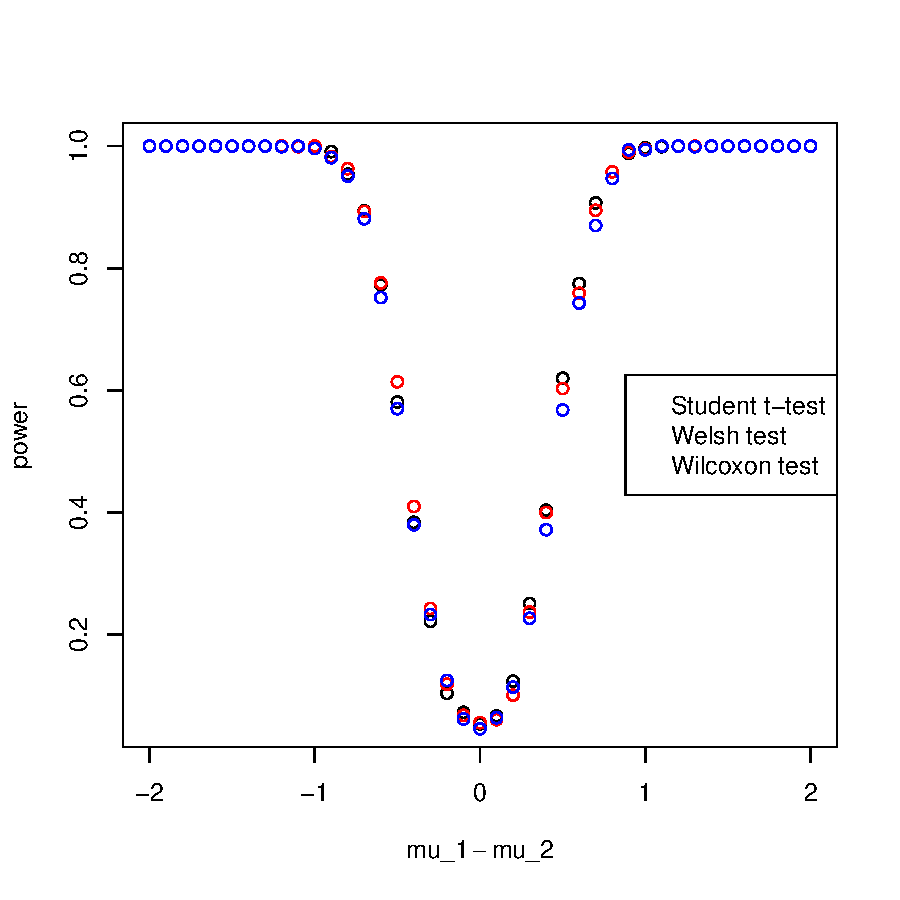
\includegraphics{p1-task_1_plot}
\label{chart_t1}
\caption{Power functions of three tests. Tests for two samples with normal distribution and equal variances.}
\end{figure}
On the first plot \ref{chart_t1} we can see that the power function looks almost the same for all tests when we consider the samples with normal distribution and equal variance. It is also shown that those test are much more efficient when the difference between means $\mu_1-\mu_2$ is nor close to 0. The power function is symetric and the values decrease significantly faster in $[-1, 1]$ interval of $\mu_1-\mu_2$. Concerning choosen significance level $\alpha=0.05$ there is no uniformly strongest test.

  \section{Task 2.}
 The second task is similar to first but instead of equal variances we have two samples, one with $\sigma=2$ and the second sample with $\sigma=4$.
\begin{Schunk}
\begin{Sinput}
>   powers_student <- vector(mode="numeric", length=0)
>   powers_welch <- vector(mode="numeric", length=0)
>   powers_wilcoxon <- vector(mode="numeric", length=0)
>   for (i in seq(-2,2,.1)){
+     powers_student = c(powers_student, t.power1(means = c(0, i), sds = c(2,4)))
+     powers_welch = c(powers_welch, t.power1(means = c(0, i), sds = c(2,4), var.equal = FALSE))
+     powers_wilcoxon = c(powers_wilcoxon, wilcoxon.power(means = c(0, i), sds = c(2,4)))
+   }